\chapter{Design issues}

In order to build the entire project around the basic algorithms, there were several
parts of the system we had to develop. We dedicate this chapter to explaining the specific
design approaches used for building each of these parts. We shall describe each of the
different components separately first and then show how they are put together in order to
obtain the final system.

The main parts of our application are the core system, the network communication module,
the parser module and the client-side graphical user interface.

\section{The core system}

The core system represents the largest part of our system as it is the one that integrates
all the algorithms presented in the previous chapter. The entire core system resides on the
client side of the application (which makes it a so-called ``fat client''). This means that
the logic of all operations described previously (such as commit, update and so on) are
handled by the client, while the repository is merely a container with support for various
simple requests. The client is the one where the processing actually takes place.

Most of the algorithms are enclosed within the methods of the Document class, while a
certain amount of them reside in the Operation class. Figure \ref{fig:coreuml} tries to
show this distribution of algorithms by presenting a class diagram of the main classes
that compose the core of the application.

\begin{figure}[htp]
\begin{center}
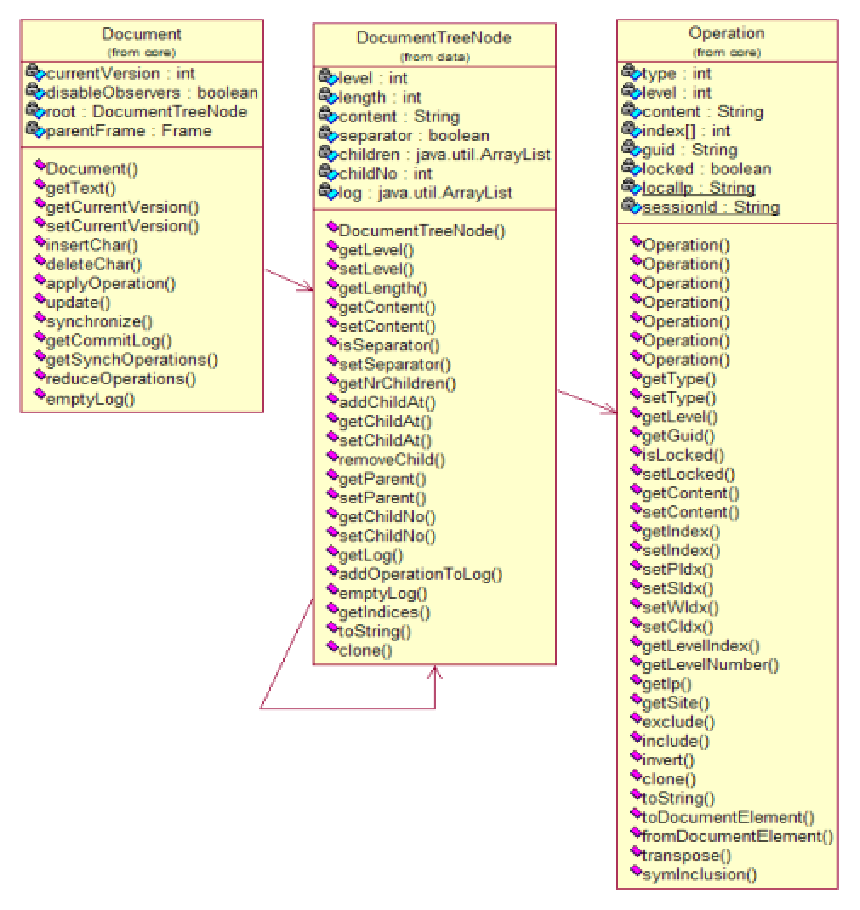
\includegraphics{img/CoreUML.eps}
\end{center}
\caption{The core system class diagram}
\label{fig:coreuml}
\end{figure}

The arrows in the figure illustrate that the Document class references a DocuementTreeNode
object as the root of the document tree and the DocumentTreeNode references a list of 
Operation objects (which form the log associated with each tree node) and also another
DocumentTreeNode object which represents the parent of the current node.

You can see that the operation transformation methods (include, exclude, transpose, symmetric
inclusion etc.) all belong to the Operation class. Also, this class provides accessors to
all of an operation's fields such as type, level, global unique identifier, content, indices
and so on.

Each DocumentTreeNode object (as the name suggests) stands for  a node in the tree that represents
the document. It is mostly a container class which additionally provides a means of managing
child nodes. The rest of the methods (both accessor and selector) are self-explaining.

A text document is represented by an instance of the Document class. Such an object provides
methods for inserting and deleting characters in and from the text document, applying
operations, updating and synchronizing this document with remote changes, obtaining the
complete log of operations which were executed on the document and clearing this log. The
way all these methods are implemented has been described in the previous chapter.

Even though the core system represents the essence of the entire application, we shall not
discuss it here any further since it has been extensively covered in chapter
\ref{chap:algorithm}. We have only mentioned it in this chapter as well in order to clarify
the general framework in which the operations already described appear.

\subsection{The XML representation of operations}

There are two methods we have not mentioned so far which appear within the Operation class
and which we would like to discuss here, namely the \emph{toDocumentElement} and the
\emph{fromDocumentElement} methods. These methods are used for creating an XML representation
of the Operation object they are called on and for recreating an Operation object from its
XML representation, respectively. The actual output (and input, respectively) of the two
methods are, in fact, DOM elements, not clear text. The DOM element generated by
\emph{toDocumentElement} will be combined with others and eventually end up written
to an XML file, while the DOM element from which an operation is recreated (by means
of \emph{fromDocumentElement}) is obtained as a subtree of a larger DOM representation
of an XML file.

The Document Type Definition (DTD) which describes how an operation is represented in XML
is reproduced below:

\begin{verbatim}
<!ELEMENT operation (guid,((pIdx)|(pIdx,sIdx)|(pIdx,sIdx,wIdx)|
  (pIdx,sIdx,wIdx,cIdx)),content)>
<!ATTLIST operation type (0|1|2) #REQUIRED>
<!ATTLIST operation level (0|1|2|3) #REQUIRED>
<!ELEMENT guid (#CDATA)>
<!ELEMENT pIdx (#CDATA)>
<!ELEMENT sIdx (#CDATA)>
<!ELEMENT wIdx (#CDATA)>
<!ELEMENT cIdx (#CDATA)>
<!ELEMENT content (#CDATA)>
\end{verbatim}

Each operation has to have its type and level represented as attributes, while the rest of
the components of the operation appear as elements (the global unique identifier, the
content and the indices). As described by the DTD, an operation can have either one, two,
three or four indices, depending on its level (document level, paragraph level, sentence
level or word level).

An example of a representation of an operation could be the following:

\begin{verbatim}
<operation type="0" level="3">
 <guid>192.168.0.1\%26e9f9:fcf46ff876:-7ffa\%26e9f9:fcf46ff876:-7ff7</guid>
 <pIdx>0</pIdx>
 <sIdx>0</sIdx>
 <wIdx>8</wIdx>
 <cIdx>6</cIdx>
 <content>s</content>
</operation>
\end{verbatim}

The operation denoted by this representation is InsertChar(0,0,8,6,'s') with the specified
global unique identifier.

\section{The network communication module}

There were several communication requirements which we wanted to meet with our application.
The most of important of these was the need for reliable communication between the clients
and the repository as well as between the clients themselves. The necessity of this 
requirement should be obvious to the reader. Imagine the simple case when a single packet
containing an operation is lost. This can have dramatic effects on the final result since
all the following operations might no longer be properly defined, leading to inconsistencies
either in the repository (if the packet was a commit packet) or in the client documents
(if the packet was a checkout or update packet). Secondly, we also aimed for a communication
mechanism which would be usable with very heterogenous environments (including firewall
protected hosts, masquaraded hosts and so on) since clients of an asynchronous system
could technically gain access to the network in very different ways.

The natural solution to these requirements was the use of the robust network communication
mechanism made available by the standard Java implementation: Remote Method Invocation. We
assume the reader is already familiar with RMI and the way it is used, so we shall only
try to describe the specific way in which we based our network module on it. Figure
\ref{fig:commuml} illustrates the RMI servers we implemented in our application.

\begin{figure}[htb]
\begin{center}
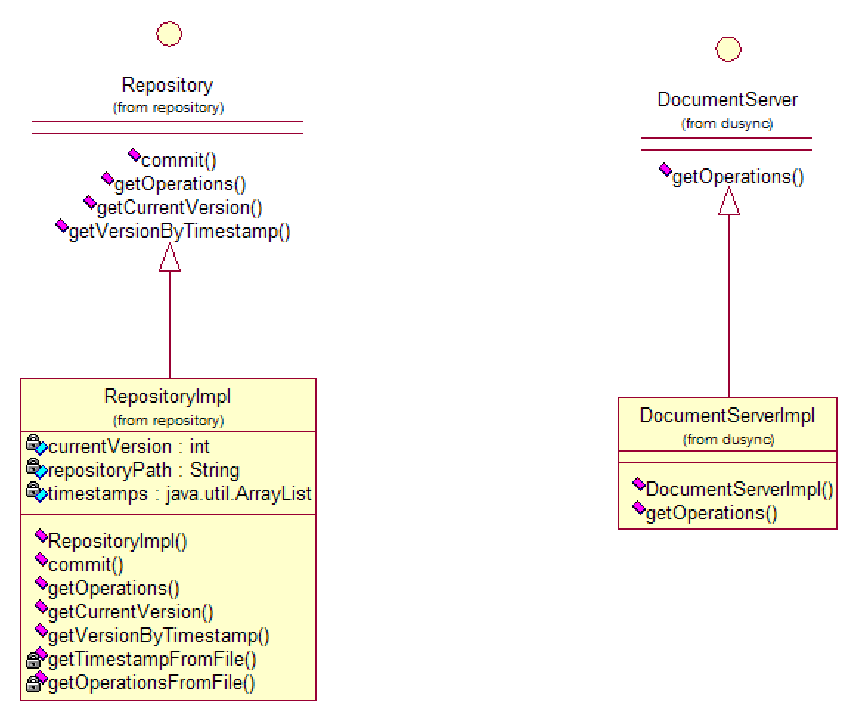
\includegraphics{img/CommUML.eps}
\end{center}
\caption{The network communication module}
\label{fig:commuml}
\end{figure}

As the figure shows, there are two distinct servers that appear in the system. One of them
is the repository server and the other is the direct user synchronization server. The
repository server is instantiated by the server side of the system and provides all the
functionality associated with the system repository. A direct user synchronization
server is instantiated on each client and has the purpose of allowing other clients to
connect to the client running the server and retrieve its operations by means of the
direct user synchronization mechanism.

The repository offers some standard functionality (represented by the \emph{getOperations},
\emph{getCurrentVersion} and \emph{commit} methods) and a more ``special'' method which allows
the clients to identify the version number closest to the a certain moment in time
(\emph{getVersionByTimestamp}). The basic functionality of the repository is to allow
its clients to store operations in the document file (by remotely calling the \emph{commit}
method) and retrieve the operations which represent the delta between two consecutive
versions (by remotely calling the \emph{getOperations} method).

Since when two or more commit operations are tried concurrently, only one should be
successful (while the others have to fail), we had to employ a mutual exclusion mechanism
which would allow us to achieve this. The solution (given the Java implementation) was to
mark the \emph{commit} operation as \emph{synchronized}, which ensured that only one client
would be able to call it at a certain moment in time. Naturally, the \emph{getCurrentVersion}
method is also \emph{synchronized} since the \emph{commit} method changes the version
number as well and it would be wrong to return an outdated version number to the clients.

As for retrieving version numbers based on timestamps, this is a fairly simple operation.
Each version is timestamped at the time it is committed with a date and time. This timestamp
is recorded in the version file along with the list of operations which comprise that
particular version. When a client wants to retrieve a certain version, (s)he usually knows
the approximate time at which it was committed. (S)he will then submit this approximate
timestamp to the repository and will expect a version number in return. The repository will
traverse the list of timestamps and will return the version number associated with the
timestamp that is closest to the one submitted by the client. Once the version number is
obtained, the client can simply perform a checkout of that particular version in order to
analyze (or even use) it.

The direct user synchronization server is slightly more simple, as the only operation it
has to support is the retrieval of the local operations. This is achieved through the
\emph{getOperations} method. The method returns all the operations that are found in the
local log of the client on which it runs (after previously locking them all - see section
\ref{sec:synch} for further details).

The rest of the network communication module is found on the clients. This part simply
connects to the RMI registry on the repository server (or on the client it wants to
synchronize with directly) and retrieves the appropriate registered remote object. Once
this is accomplished, RMI allows clients to call the methods of the remote object as if
they were local.

The configuration of the RMI server (i.e., its IP address and port) are manageable by the
client by means of the graphical user interface.

\subsection{XML representation of document versions}
\label{sec:xmlop}

Returning to the repository server, the final aspect to mention is the XML representation
used to store version files. Each set of operations which comprise the change between two
consecutive versions is stored in a separate XML file which is described by the following
DTD:

\begin{verbatim}
<!DOCTYPE version-update [
  <!ELEMENT version-update (timestamp,operation+)>
  <!ELEMENT timestamp (year,month,day,hour,minute,second,mili)>
  <!ELEMENT year (#CDATA)>
  <!ELEMENT month (#CDATA)>
  <!ELEMENT day (#CDATA)>
  <!ELEMENT hour (#CDATA)>
  <!ELEMENT minute (#CDATA)>
  <!ELEMENT second (#CDATA)>
  <!ELEMENT mili (#CDATA)>
  <!ELEMENT operation ...>
]>
\end{verbatim}

The ``operation'' element has already been described in section \ref{sec:xmlop} and therefore
has not been repeated here. As you can see, a version update consists of a single timestamp
identifying the moment in time at which it has been committed followed by a list of one or
more operations. An example of such a version update could be the following:

\begin{verbatim}
<?xml version="1.0" encoding="UTF-8"?>
<version-update>
  <timestamp>
    <year>2004</year><month>6</month><day>5</day>
    <hour>14</hour><minute>2</minute><second>43</second><milli>265</milli>
  </timestamp>
  <operation type="1" level="0">
    <guid>192.168.0.1\%cafb56:fcf4795cd1:-7ffa\%cafb56:fcf4795cd1:-7ff0</guid>
    <pIdx>7</pIdx>
    <content>This is a test.</content>
  </operation>
  <operation type="1" level="0">
    <guid>192.168.0.1%cafb56:fcf4795cd1:-7ffa%cafb56:fcf4795cd1:-7fef</guid>
    <pIdx>5</pIdx>
    <content>This is another test.</content>
  </operation>
</version-update>
\end{verbatim}

This represents a commit consisting of two operations, both of the type InsertParagraph. The
version number itself is stored in the name of the XML file. This is a trick used in order
to be able to quickly retrieve the version changes particular to a specific version without
having to traverse a (possibly) large number of files. By using the version number as part
of the file name of the XML file, we can simply go directly to the correct file when a
request is made by a client.

\section{The parser module}

One of the other important parts of our application resides in the module which deals with
the generation of a tree document representation of a random text (transforming a linear
structure - the text stream - into a hierarchical one - the tree representation of the
document using DocumentTreeNode objects as nodes in the tree). This is what we call
the parser module. Its entire functionality resides in a single class which is illustrated
in figure \ref{fig:parseruml}.

\begin{figure}[htb]
\begin{center}
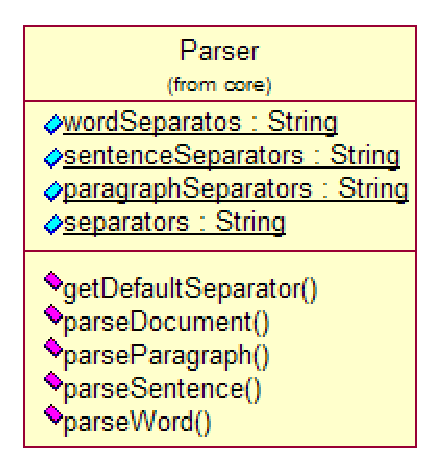
\includegraphics{img/ParserUML.eps}
\end{center}
\caption{The parser class}
\label{fig:parseruml}
\end{figure}

The function of this class is to parse either an entire document, a paragraph, a sentence
or merely a single word from a text stream. If we speak of a document, the parsing is done
until the end of the stream is reached. If, on the other hand, we speak of lower level
semantic units, the parsing is done either until a separator specific for that semantic
unit is reached or the end of the stream is reached.

The functionality of the parser is based on the assumption that all texts are strings in
the language defined by the following grammar (described in BNF):

\begin{verbatim}
document ::= paragraph document |
             ""

paragraph ::= actual_paragraph |
              paragraph_separator

actual_paragraph ::= sentence actual_paragraph |
                     sentence

paragraph_separator ::= "\n" | "\r"

sentence ::= actual_sentence |
             sentence_separator

actual_sentence ::= word actual_sentence |
                    word

sentence_separator ::= "." | "!" | "?"

word ::= actual_word |
         word_separator

actual_word ::= character actual_word |
                character

word_separator ::= " " | "," | ";" | ":"

character ::= any_charcter_other_than_separators
\end{verbatim}

The main aspect we would like to underline here is that semantic unit separators (paragraph
separators, sentence separators and word separators) are treated similarly to the semantic
units they separate, i.e. each paragraph separator is viewed as a separate paragraph, each
sentence separator is viewed as a separate sentence and each word separator is viewed as a
separate word.

Based on this grammar, the \emph{parseDocument} method parses an entire text document
generating paragraph, sentence, word and character nodes which correspond to the actual
structure of the text. But this way of generating the document tree representation is
less used in our project. Instead, as the document is usually generated by successively
applying the operations received from the repository and as these operations insert at
most full paragraphs, the document tree representation is built progressively by creating
entire subtrees which represent either a paragraph, a sentence or a word using the
appropriate \emph{parseXXX} method of the Parser class and adding them (the subtrees)
in the correct position in the tree.

Apart from the parser, two other methods relevant to the management of the document
tree representation are the \emph{insertChar} and \emph{deleteChar} functions from
the Document class. These deal with the local insertions and deletions of single characters
(as opposed to modifying the document by means of applying remotely generated operations).
Each insertion may simply modify the content of a word node (if the user inserts a
character in an existing word), create a new word node (if the user inserts a word
separator or the first character of a new word), create a new sentence node (if the
user inserts a sentence separator or the first character of a new sentence) or create
a new paragraph node (if the user inserts a paragraph separator or the first character
of a new paragraph). In the case of inserting the first character of a new paragraph
or sentence there are actually three (or two nodes, respectively) that are being built,
not just one. This is because when a new paragraph is created the first sentence and first word of
that paragraph are also created and when a new sentence is created the first word of that
sentence is also created. Deletion takes place in the same way: when a character is
deleted, depending on whether it is the last character of a word/sentecence/paragraph
or not, the appropriate operations are generated and the appropriate node(s) is(are)
deleted.

\section{The Graphical User Interface}

Finally, the last piece of the puzzle consists of the client side graphical user interface
which allows the user to perform a series of actions, among which the most important are:

\begin{itemize}

\item edit a text document
\item commit the changes made to a text document
\item update the local working copy with the changes committed by others
\item check out a particular version of a document from the repository
\item choose the granularity level to work at
\item choose the conflict resolution policy to be used
\item manage a list of users with whom direct synchronization can be employed
\item synchronize with any user from the list mentioned above

\end{itemize}

All these should be performed in a simple, intuitive manner which is exactly what
we tried to accomplish with our graphical user interface. Figure \ref{fig:guiuml} is a
representation of the class diagram which contains the main GUI components. Aside from
the ones represented in the figure, the system also contains some additional GUI-related
classes which have not been represented due to lack of space.

\begin{figure}[htp]
\begin{center}
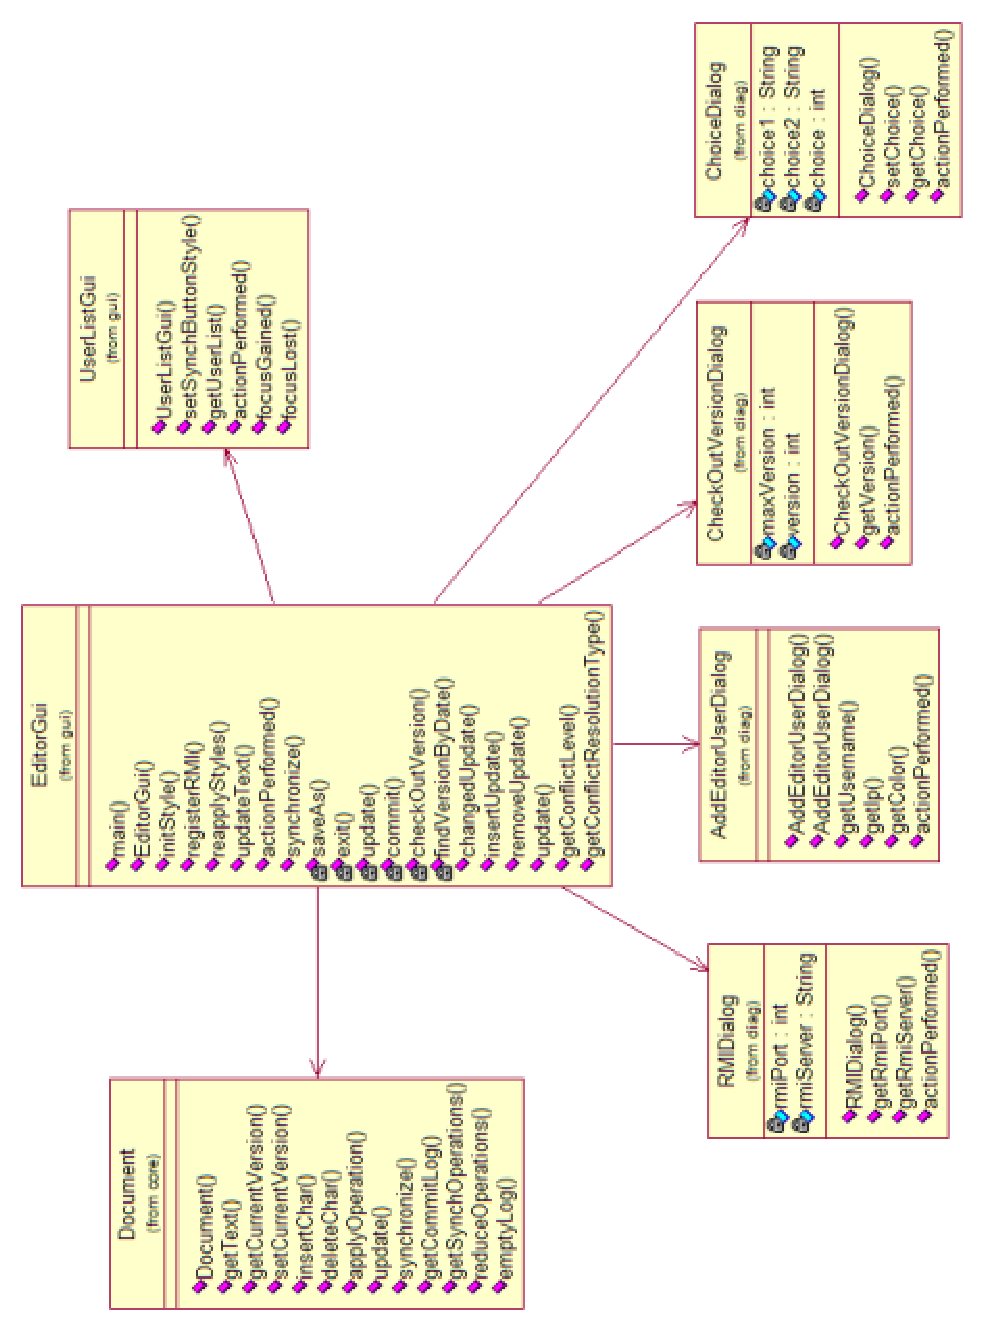
\includegraphics{img/EditorGuiUML.eps}
\end{center}
\caption{The graphical user interface}
\label{fig:guiuml}
\end{figure}

The figure also shows the Document class once again in order to illustrate that this
is actually the so-called ``data model'' of the graphical user interface, as the entire
functionality of the GUI strongly relates and interacts with an instance of the Document
class. Every change or action the user performs by means of the GUI is actually reflected
in the state of the Document instance used. The GUI basically provides a way to control
the parameters of the Document instance and to trigger the various methods which determine
changes in the document.

Aside from the main GUI, the figure also shows a few classes called \emph{XXXDialog}. These
all represent separate screens which allow the user to perform various actions such as
choosing the repository server to use, managing the list of users (s)he wishes to
directly synchronize with, choosing between document variants in case of conflict and so
on.

All in all, the GUI is a fairly simple one which allows the user to perform all the actions
allowed by the system. We have also attached a screen shot of our graphical user interface
(figure \ref{fig:screenshot}) so that the reader can also visualize this component of
the system put to work.

\begin{figure}[htp]
\begin{center}
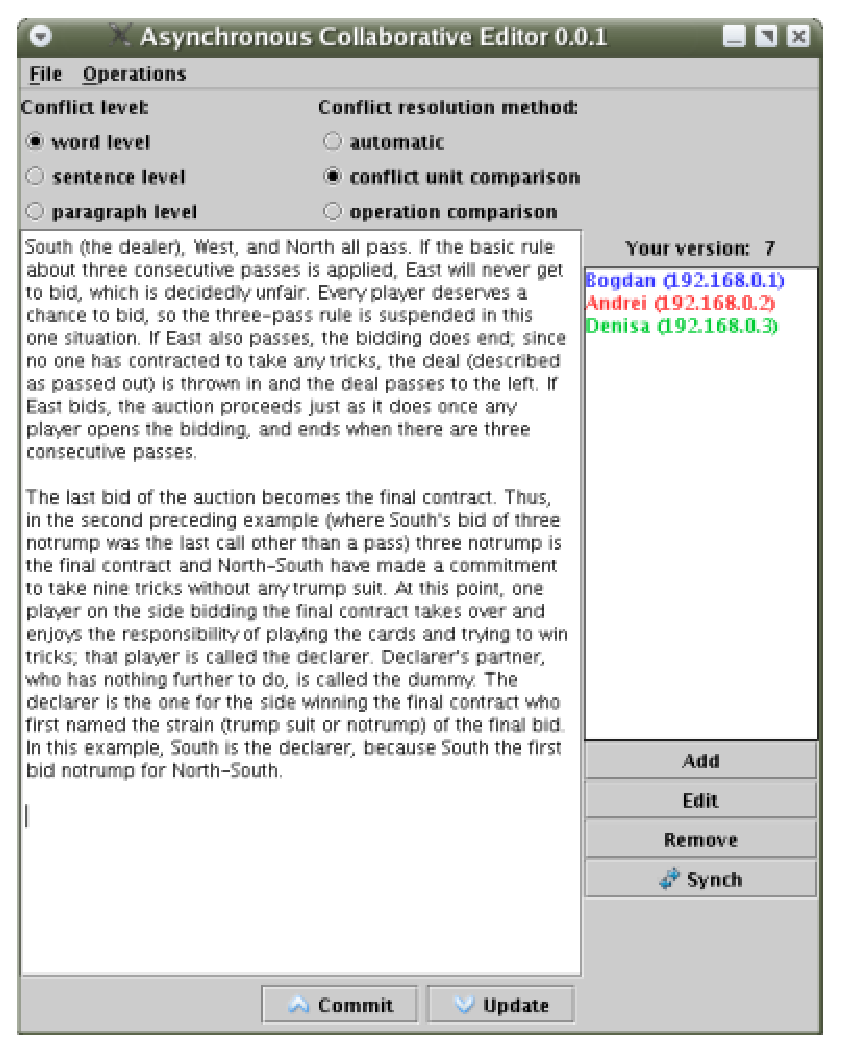
\includegraphics{img/screenshot.eps}
\end{center}
\caption{A screen shot of the client GUI}
\label{fig:screenshot}
\end{figure}

\section{Putting it all together}

As all the subsystems of our application have been briefly introduced, let us now
illustrate how they all work together in order to provide a fully-functional and integrated
system. We do this by means of the following figure:

\begin{figure}[htb]
\begin{center}
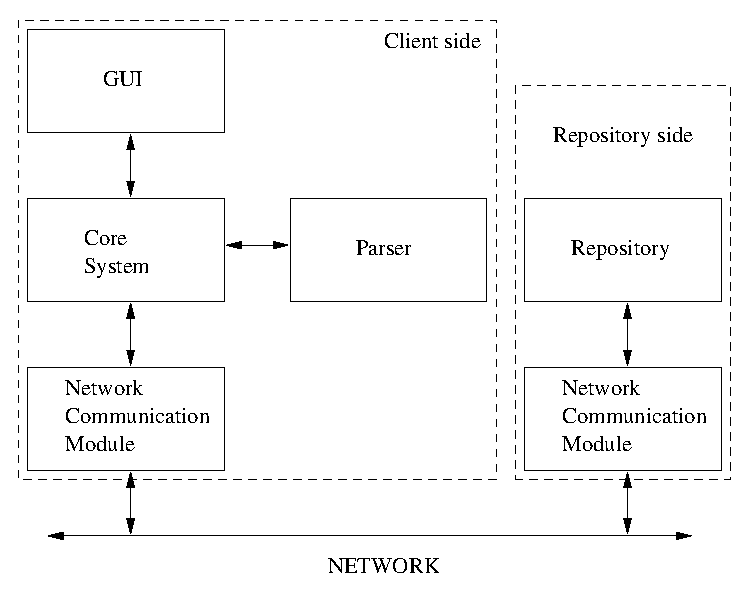
\includegraphics{img/system.eps}
\end{center}
\caption{The entire system}
\label{fig:system}
\end{figure}

The figure illustrates that the client side is governed by the core system which is the
central part of the system. The GUI is a ``wrapper'' over the core system which allows
the editing of the text document and ensures a simplified user control over the core
system. The parser module is used by the core system in order to transform linear
representations of text into equivalent tree representations. The communication (over
any network) between the client and the repository is achieved by the network communication
module.

The functioning of all of the subsystems that appear in the figure has been described
in the previous sections of this chapter. The overall architecture is highly modular and,
consequently, easy to extend. This means that the tree structure can be changed, the
operation set can be enlarged with new operations and the GUI (for various reasons) could be
redesigned without any influence on the other modules.

All in all, we have adopted a modern, modular, architecture in the application built
around our core system, the final purpose of which was to allow users to benefit from
the performance improvements we provide. The architecture, however, came second
in our efforts as the largest amount of time was allocated for the development of
the algorithms described in the previous chapter.